%----------------------------------------------------------------------------------------
%	PACKAGES AND THEMES
%----------------------------------------------------------------------------------------

\documentclass{beamer}

\mode<presentation> {
\usetheme{Madrid}

\setbeamertemplate{navigation symbols}{} % To remove the navigation symbols from the bottom of all slides uncomment this line
}

% German Language Settings
\usepackage[utf8]{inputenc}
\usepackage[ngerman]{babel}

\usepackage{graphicx} % Allows including images
\usepackage{booktabs} % Allows the use of \toprule, \midrule and \bottomrule in tables
\usepackage{hyperref} % For Table of Content in PDF



\newcommand{\backupbegin}{
   \newcounter{finalframe}
   \setcounter{finalframe}{\value{framenumber}}
}
\newcommand{\backupend}{
   \setcounter{framenumber}{\value{finalframe}}
}

%----------------------------------------------------------------------------------------
%	TITLE PAGE
%----------------------------------------------------------------------------------------

\title[Short title]{Full Title of the Talk} % The short title appears at the bottom of every slide, the full title is only on the title page

\author{Ramil Sabirov, Joel Choi, Eric Remigius} % Your name
\institute[RWTH] % Your institution as it will appear on the bottom of every slide, may be shorthand to save space
{
RWTH Aachen \\ % Your institution for the title page
\medskip
\textit{Gruppe3} % Your email address
}
\date{\today} % Date, can be changed to a custom date

\begin{document}

\begin{frame}
\titlepage % Print the title page as the first slide
\end{frame}

%----------------------------------------------------------------------------------------
%	PRESENTATION SLIDES
%----------------------------------------------------------------------------------------

%------------------------------------------------
\section{Task 1 & 2}
%------------------------------------------------

\begin{frame}
\frametitle{Aufbau der Paranoid-Baumsuche}
Wir nutzen folgende Player (Methoden):
\begin{enumerate}
\item[•] Starting Max-Player
\item[•] Max-Player
\item[•] Min-Player
\end{enumerate}\hfill\break
Mit den Aufgaben:
\begin{enumerate}
\item[•] \textbf{Starting Max-Player:} wie Max-Player, aktualisiert jedoch den aktuell besten Zug
\item[•] \textbf{Max-Player:} maximiert den Stellungswert über die Möglichkeiten
\item[•] \textbf{Min-Player:} minimiert den Stellungswert über die Möglichkeiten
\end{enumerate}

\end{frame}

%------------------------------------------------

\begin{frame}
\frametitle{Callgraph der Algorithmen}


\begin{center}
	\includegraphics[scale=0.2]{figures/MinMaxCallGraph.pdf}
\end{center}

\end{frame}

%------------------------------------------------
\section{Task 3}
%------------------------------------------------

\begin{frame}
\frametitle{Performance Tools}

  \begin{figure}
    \centering
    \includegraphics[width=\textwidth]{figures/ClassDiagrammPerfLogging.pdf}
  \end{figure}

\end{frame}

%------------------------------------------------

\begin{frame}
\frametitle{Performance Ergebnisse Tiefe 1 (Zeit)}
  \begin{figure}
    \centering
    \includegraphics[scale=0.4]{figures/time-1.pdf}
  \end{figure}

\end{frame}

%------------------------------------------------

\begin{frame}
\frametitle{Performance Ergebnisse Tiefe 1 (Knoten)}
  \begin{figure}
    \centering
    \includegraphics[scale=0.8]{figures/node-1.pdf}
  \end{figure}

\end{frame}

%------------------------------------------------

\begin{frame}
\frametitle{Performance Ergebnisse Tiefe 2 (Zeit)}
  \begin{figure}
    \centering
    \includegraphics[scale=0.4]{figures/time-2.pdf}
  \end{figure}

\end{frame}

%------------------------------------------------

\begin{frame}
\frametitle{Performance Ergebnisse Tiefe 2 (Knoten)}
  \begin{figure}
    \centering
    \includegraphics[scale=0.8]{figures/node-2.pdf}
  \end{figure}

\end{frame}

%------------------------------------------------
\begin{frame}
\frametitle{Performance Ergebnisse Tiefe 3 (Zeit)}
  \begin{figure}
    \centering
    \includegraphics[scale=0.4]{figures/time-3.pdf}
  \end{figure}

\end{frame}

%------------------------------------------------

\begin{frame}
\frametitle{Performance Ergebnisse Tiefe 3 (Knoten)}
  \begin{figure}
    \centering
    \includegraphics[scale=0.8]{figures/node-3.pdf}
  \end{figure}

\end{frame}

%------------------------------------------------
%------------------------------------------------
\appendix
\backupbegin
%------------------------------------------------

\begin{frame}
\frametitle{Fragen und Rückmeldung}
  \begin{itemize}
    \item<1-> Reports kommen sehr spät, Anmerkungen meist schon umgesetzt
    \item<2-> Ist es erlaubt/sinnvoll eine Map-Datenbank zu führen?
  \end{itemize}
\end{frame}

%----------------------------------------------------------------------------------------
\backupend
%----------------------------------------------------------------------------------------

\end{document} 